%!TEX program = xelatex

\documentclass[a4paper]{ctexart}

%% 导言区
%% geometry for A4 paper, word preference
\usepackage{geometry}
\geometry{
  left=20.0mm,
  right=20.mm,
  top=10mm,
  bottom=20.0mm
}
%% for font 
\usepackage{xeCJK}
%\newcommand{\song}{\CJKfamily{song}}
%\newcommand{\kai}{\CJKfamily{kai}}

%% author
\newcommand{\me}[2]{
  \author{
    {\bfseries 姓名:}\underline{#1}\hspace{2em}
    {\bfseries 邮箱:}\underline{#2}\hspace{2em}
  }
}

%% for picture
\usepackage{graphicx}

%% for math
\usepackage{amsmath,ntheorem}
\theoremstyle{break} %标题换行
%\theorembodyfont{\song}
%\theoremheaderfont{\kai\bfseries}
\newtheorem*{problem}{\Large{题目}}[subsection]

\newenvironment{solution}
{
	\textbf{\Large{解答:}}\\
}   

%% for pseudocode
\usepackage{algorithm}
\usepackage{algpseudocode}

\algblockdefx[SWITCH]{Switch}{EndSwitch}
  [1]{\bf{Switch :} #1}
  [0]{\bf{EndSwitch}}
\algblockdefx[CASE]{Case}{EndCase}%
  [1]{\bf{Case :} #1}%
  [0]{\bf{EndCase} }


%% algorithm分页
\makeatletter
\newenvironment{breakablealgorithm}
  {% \begin{breakablealgorithm}
    \begin{center}
      \refstepcounter{algorithm}% New algorithm
      \hrule height.8pt depth0pt \kern2pt% \@fs@pre for \@fs@ruled
      \renewcommand{\caption}[2][\relax]{% Make a new \caption
        {\raggedright\textbf{\ALG@name~\thealgorithm} ##2\par}%
        \ifx\relax##1\relax % #1 is \relax
          \addcontentsline{loa}{algorithm}{\protect\numberline{\thealgorithm}##2}%
        \else % #1 is not \relax
          \addcontentsline{loa}{algorithm}{\protect\numberline{\thealgorithm}##1}%
        \fi
        \kern2pt\hrule\kern2pt
      }
  }{% \end{breakablealgorithm}
      \kern2pt\hrule\relax% \@fs@post for \@fs@ruled
    \end{center}
  }
\makeatother
  


\title{编译原理作业 (1)参考答案}
\me{王腾}{171240540@smail.nju.edu.cn}

%% 正文区
\begin{document}
\maketitle

\begin{problem}[手写词法分析器]
    根据下面的状态转移图以及课上介绍的识别方法, 给出识别数字
    (正整数、不带科学计数法的浮点数以及带科学计数法的浮点数)的伪代码。

    {\centering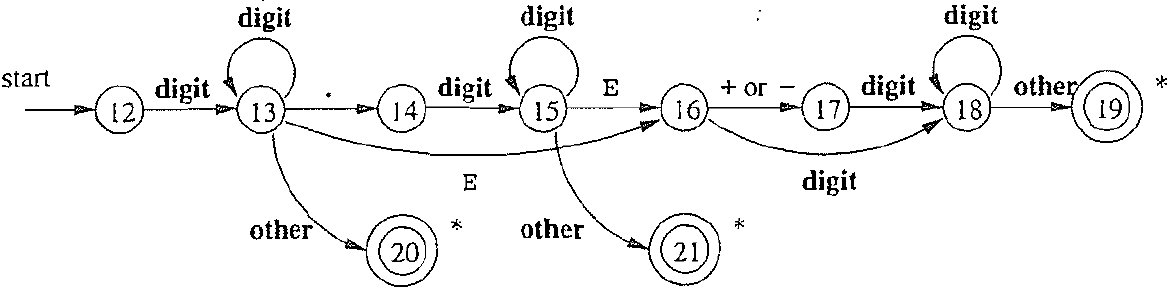
\includegraphics[width=0.70\textwidth]{figs/number} }
\end{problem}
\begin{solution}
  \bfseries{如果发现问题,希望指出错误发送到我邮箱,谢谢!}
  \begin{breakablealgorithm}

    \caption{Parser}
    \begin{algorithmic}[1]
    \Procedure{Parse}{$str$}\Comment{$str$ is input stream and suppose it has a end character EOF}
    \State $l \gets 1, r\gets 1$\Comment{left and right bound of lexeme}
    \State $state\gets 12$\Comment{simulate the procedure of the diagram}
    \State $fstate\gets 0$\Comment{to decide final state when goes back}
    \While{$r\le str.length$}\Comment{$str.length$ includes EOF, each loop $r$ increases one}
    \Switch{$state$}
    %% 12
      \Case{$12$}
        \If{$isdigit(str[r])$}
          \State $state\gets 13$
        \Else
          \State $l\gets l+1$\Comment{skip mysterious character}
        \EndIf
        \State $break$\Comment{begin next loop}
      \EndCase
    %% 13
      \Case{$13$}
        \If{$isdigit(str[r])$}
          \State $state\gets 13$
        \ElsIf{$str[r]=='.'$}
          \State $state\gets 14$
        \ElsIf{$str[r]=='E'$}
          \State $state\gets 16$
        \Else
          \State $state\gets 20$
        \EndIf 
        \State $fstate\gets 20$\Comment{set final state for going back}
        \State $break$       
      \EndCase
    %% state 14
      \Case{$14$}
        \If{$isdigit(str[r])$}
          \State $state\gets 15$
        \Else
          \State $state\gets fstate$
          \State $r\gets r-2$
        \EndIf 
        \State $break$       
      \EndCase
    %% 15
      \Case{$15$}
        \If{$isdigit(str[r])$}
          \State $state\gets 15$
        \ElsIf{$str[r]=='E'$}
          \State $state\gets 16$
        \Else
          \State $state\gets 21$
        \EndIf 
        \State $fstate\gets 21$
        \State $break$       
      \EndCase
    %% 16
      \Case{$16$}
        \If{$isdigit(str[r])$}
          \State $state\gets 18$
        \ElsIf{$str[r]=='+'\text{ \bf{or} } str[r]=='-'$}
          \State $state\gets 17$
        \Else
          \State $r\gets r-2$
          \State $state\gets fstate$
        \EndIf 
        \State $break$       
      \EndCase
    %% 17
      \Case{$17$}
        \If{$isdigit(str[r])$}
          \State $state\gets 18$
        \Else
          \State $r\gets r-3$
          \State $state\gets fstate$
        \EndIf 
        \State $break$       
      \EndCase      
    %% 18
      \Case{$18$}
        \If{$isdigit(str[r])$}
          \State $state\gets 18$
        \Else
          \State $state\gets 19$
        \EndIf 
        \State $fstate\gets 19$
        \State $break$       
      \EndCase   
    %% 19 20 21
      \Case{$19$ \bf{or} $20$ \bf{or} $21$}
        \State $print(str[l-r])$\Comment{print from $str[l]$ to $str[r]$}
        \State $l\gets r+1$
        \State $state\gets 12$
        \State $fstate\gets 0$
        \State $break$       
      \EndCase     
    \EndSwitch
    %% r++
    \State $r\gets r+1$\Comment{one loop check one character}
    \EndWhile
    \EndProcedure
    \end{algorithmic}

  \end{breakablealgorithm}
\end{solution}
%%%%%%%%%%%%%%%

\end{document}